\documentclass[10pt,a4paper]{article}

\newcommand{\DocumentTitle}{Technical Documentation}

\usepackage[a4paper,left=17mm,right=17mm,top=26mm,bottom=21mm,headheight=20pt,headsep=10mm]{geometry}
\usepackage{fix-cm}
\usepackage{fontspec}
\setmainfont{texgyreheros-regular.otf}[BoldFont=texgyreheros-bold.otf,ItalicFont=texgyreheros-italic.otf]
\setmonofont{lmmono10-regular.otf}
\usepackage[table]{xcolor}
\usepackage{array,booktabs,ragged2e}
\newcolumntype{L}[1]{>{\raggedright\arraybackslash}p{\dimexpr #1\linewidth-2\tabcolsep\relax}}
\usepackage{amsmath}
\usepackage{tikz}
\usetikzlibrary{arrows.meta,positioning}
\usepackage{fancyhdr,lastpage}
\usepackage{fancyvrb}
\usepackage{titlesec}
\usepackage{hyperref}
\definecolor{Navy}{HTML}{112744}
\definecolor{Blue}{HTML}{2463AD}
\definecolor{Ink}{HTML}{23354C}
\definecolor{Muted}{HTML}{586A80}
\definecolor{Pale}{HTML}{EDF4FC}
\definecolor{Stripe}{HTML}{F5F8FC}
\definecolor{Border}{HTML}{DCE5EF}
\definecolor{Amber}{HTML}{FFF5E4}
\hypersetup{colorlinks=true,urlcolor=Blue,linkcolor=Blue,pdftitle={BizWizard - \DocumentTitle},pdfauthor={BizWizard project}}
\pagestyle{fancy}
\fancyhf{}
\fancyhead[L]{\textcolor{Blue}{\bfseries BW}\quad\textcolor{Navy}{\bfseries BizWizard}}
\fancyhead[R]{\footnotesize\textcolor{Muted}{\DocumentTitle\ | Topic E}}
\fancyfoot[L]{\scriptsize\textcolor{Muted}{BizWizard | \DocumentTitle}}
\fancyfoot[R]{\scriptsize\textcolor{Muted}{\thepage\ / \pageref*{LastPage}}}
\renewcommand{\headrulewidth}{0pt}
\renewcommand{\footrulewidth}{0.3pt}
\renewcommand{\footrule}{\hbox to\headwidth{\color{Border}\leaders\hrule height \footrulewidth\hfill}}
\setlength{\parindent}{0pt}
\setlength{\parskip}{6pt}
\setlength{\emergencystretch}{2em}
\raggedbottom
\AtBeginDocument{\fontsize{10}{14}\selectfont\color{Ink}\raggedright}
\titleformat{\subsection}{\color{Navy}\bfseries\fontsize{12}{16}\selectfont}{}{0pt}{}
\titlespacing*{\subsection}{0pt}{9pt}{4pt}
\newcommand{\DocSection}[3]{%
  {\color{Blue}\bfseries\fontsize{9}{12}\selectfont #1\par}\vspace{5pt}%
  {\color{Navy}\bfseries\fontsize{24}{28}\selectfont #2\par}\vspace{3pt}%
  {\color{Muted}\fontsize{10.5}{15}\selectfont #3\par}\vspace{6pt}}
\newcommand{\SmallText}[1]{{\color{Muted}\fontsize{8.5}{11.5}\selectfont #1\par}}
\newcommand{\EvidenceFile}[1]{\href{https://github.com/mahfuz-saim/bizwizard/blob/main/evidence/submission/#1}{\nolinkurl{#1}}}
\newcommand{\EvidenceRevision}{\SmallText{Recorded on 18 October 2026 (UTC), from clean revision \texttt{8f394d2d074b}. These are saved results, not a fresh test of the current release. Each JSON report includes the full revision and source hashes.}}
\newcommand{\DocNote}[2][Pale]{%
  \par\begingroup\setlength{\fboxsep}{9pt}%
  \colorbox{#1}{\parbox{\dimexpr\linewidth-18pt\relax}{\raggedright #2}}\endgroup\par}
\newenvironment{ReportTable}[1]{%
  \par\begingroup\fontsize{9.2}{12.5}\selectfont%
  \setlength{\tabcolsep}{6pt}\setlength{\extrarowheight}{4pt}%
  \renewcommand{\arraystretch}{1.12}%
  \rowcolors{2}{white}{Stripe}\begin{tabular}{#1}}
  {\end{tabular}\endgroup\par}
\DefineVerbatimEnvironment{CodeBlock}{Verbatim}{fontsize=\footnotesize,frame=single,framerule=0.4pt,framesep=8pt,rulecolor=\color{Border},xleftmargin=0pt,xrightmargin=0pt}
\tikzset{docbox/.style={draw=Border,fill=Pale,rounded corners=4pt,align=left,inner sep=8pt,text width=0.265\linewidth,font=\fontsize{8.5}{11.5}\selectfont},flow/.style={-{Stealth[length=4pt]},draw=Blue,line width=0.8pt}}
\newcommand{\ArchitectureDiagram}{%
\begin{center}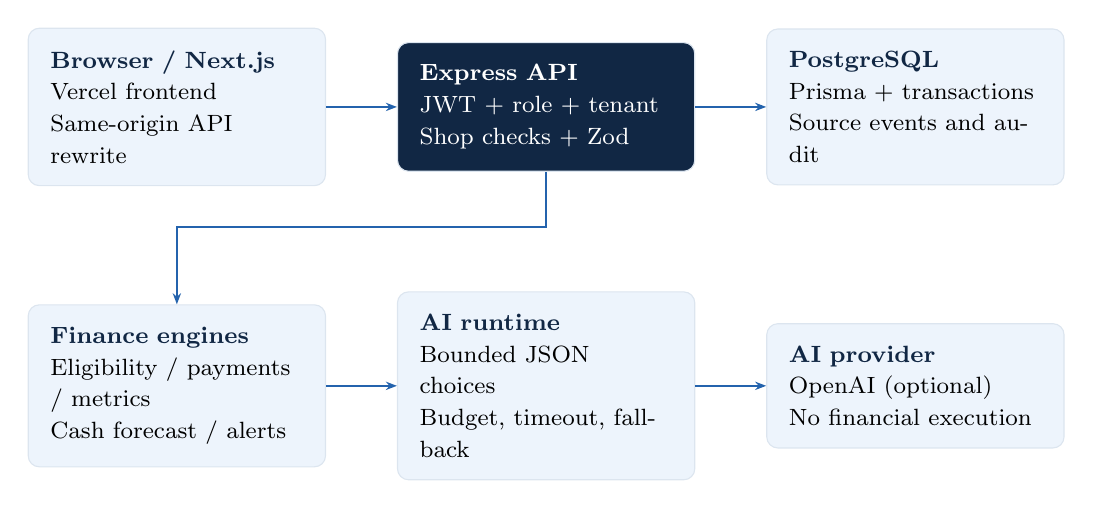
\begin{tikzpicture}[node distance=15mm and 9mm]
  \node[docbox] (browser) {\textcolor{Navy}{\bfseries Browser / Next.js}\\Vercel frontend\\Same-origin API rewrite};
  \node[docbox,right=of browser,fill=Navy,text=white] (api) {\bfseries Express API\normalfont\\JWT + role + tenant\\Shop checks + Zod};
  \node[docbox,right=of api] (db) {\textcolor{Navy}{\bfseries PostgreSQL}\\Prisma + transactions\\Source events and audit};
  \node[docbox,below=of browser] (rules) {\textcolor{Navy}{\bfseries Finance engines}\\Eligibility / payments / metrics\\Cash forecast / alerts};
  \node[docbox,right=of rules] (ai) {\textcolor{Navy}{\bfseries AI runtime}\\Bounded JSON choices\\Budget, timeout, fallback};
  \node[docbox,right=of ai] (external) {\textcolor{Navy}{\bfseries AI provider}\\OpenAI (optional)\\No financial execution};
  \draw[flow] (browser)--(api);\draw[flow] (api)--(db);
  \draw[flow] (api.south)--++(0,-7mm)-|(rules.north);
  \draw[flow] (rules)--(ai);\draw[flow] (ai)--(external);
\end{tikzpicture}\end{center}
\SmallText{Trust boundaries: browser | application/VPS | database | optional external providers}}
\newcommand{\EvaluationDiagram}{%
\begin{center}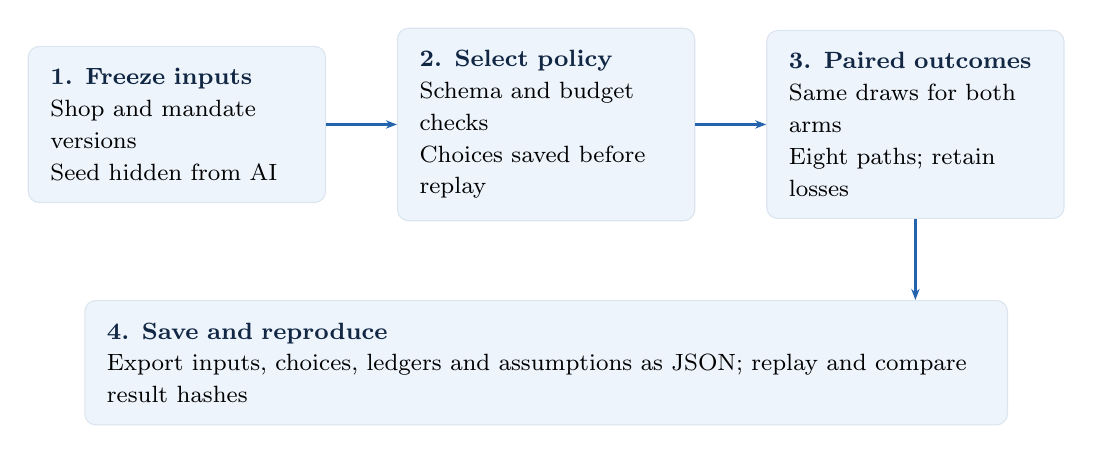
\begin{tikzpicture}[node distance=9mm]
  \node[docbox] (inputs) {\textcolor{Navy}{\bfseries 1. Freeze inputs}\\Shop and mandate versions\\Seed hidden from AI};
  \node[docbox,right=of inputs] (choices) {\textcolor{Navy}{\bfseries 2. Select policy}\\Schema and budget checks\\Choices saved before replay};
  \node[docbox,right=of choices] (outcomes) {\textcolor{Navy}{\bfseries 3. Paired outcomes}\\Same draws for both arms\\Eight paths; retain losses};
  \node[docbox,below=10mm of choices,text width=0.92\linewidth] (export) {\textcolor{Navy}{\bfseries 4. Save and reproduce}\\Export inputs, choices, ledgers and assumptions as JSON; replay and compare result hashes};
  \draw[flow] (inputs)--(choices);\draw[flow] (choices)--(outcomes);\draw[flow] (outcomes.south)--(outcomes.south |- export.north);
\end{tikzpicture}\end{center}}


\begin{document}

\DocSection{01 / OVERVIEW}{Technical Documentation}{2026 FinTechathon International Track\newline Topic E - SME Finance Copilot}

\DocNote{\textbf{Purpose.} Help a small-business owner compare financing, anticipate cash pressure and understand business performance. Financial calculations remain deterministic; AI selects or explains constrained options.}

\subsection*{Implemented capabilities}

\begin{ReportTable}{L{0.289421}L{0.710579}}

\rowcolor{Navy} \textcolor{white}{\textbf{Topic E capability}} & \textcolor{white}{\textbf{Implemented workflow}} \\

Financing-option matching & Build a shop profile; apply eligibility rules; rank feasible products; price and negotiate simulated offers; create an owner-approved application and repayment schedule. \\

Cash-flow management & Maintain cash events and commitments; project a 90-day balance; raise rule-based alerts; propose guarded treasury actions and link recorded collection evidence. \\

Business financial analysis & Compute product economics and working-capital metrics; verify candidate explanations; compare scenarios; measure 30-day observations and matched sandbox outcomes. \\

\end{ReportTable}

\subsection*{Assessment criteria}

\textbf{Task completion (40\%):} the three workflows and their execution evidence. \textbf{Security \& compliance (30\%):} authorization, financial guards and risk assessment. \textbf{Innovation \& interaction (30\%):} structured AI choices, policy-based negotiation, editable mandates and reproducible paired evaluations.


\subsection*{Scope}

The application is a sandbox finance copilot. Financing offers and money movement are simulated; no external lender is contacted and no bank transfer is executed. This document describes the implemented workflows, evaluation methods and operating limitations.


\textbf{Application:} \url{https://bizwizard.sadman.app}\newline \textbf{Repository:} \url{https://github.com/mahfuz-saim/bizwizard}\newline Reviewer access is required for the private repository.


\clearpage

\DocSection{02 / ARCHITECTURE}{System Architecture}{Application components, data flow and trust boundaries.}

\ArchitectureDiagram

\subsection*{Security design and data flow}

The browser sends authenticated requests to the frontend's same-origin /api/proxy/v1 rewrite. Next.js forwards to the configured backend. Express verifies the token and required role, checks tenant membership and employee shop assignment, validates the request, then invokes a scoped service. CORS is not the authorization boundary.


\begin{ReportTable}{L{0.213573}L{0.786427}}

\rowcolor{Navy} \textcolor{white}{\textbf{Layer}} & \textcolor{white}{\textbf{Responsibility}} \\

Presentation & Next.js / React / Tailwind; dashboard workflows, light/dark themes, loading states and owner/employee controls. Hidden buttons are convenience, not access control. \\

Finance service & Matching, cash flow, analysis, agent ledger and simulator modules. Pure TypeScript engines calculate money and constraints; service transactions persist approved state. \\

Persistence & One production PostgreSQL database managed through Prisma migrations. Sales, debts, lots and expenses feed finance records; policy versions, decisions, runs and evaluation ledgers support traceability. \\

\end{ReportTable}

The disposable local simulator\_test database is test infrastructure, not a second required production database. In-app demo workspaces are separate, scoped shops copied from a source shop; a virtual clock isolates simulated dates. Source history must remain unchanged through copy, run and reset.


\SmallText{Key record families: FinancingOffer / Application / LoanSchedule; CashAccount / Transaction / Commitment / Alert / TreasuryAction; Insight / Scenario / CapitalDecision; AiAgentPolicy / AiDecision / AiRun / FinanceEvaluation. This is not full double-entry or bank-reconciled accounting. Upload and push integrations are separate backend services, outside the finance path shown above.}

\clearpage

\DocSection{03 / FINANCING}{Financing Algorithms}{Eligibility, affordability, offer ranking and bounded negotiation.}

\begin{ReportTable}{L{0.261477}L{0.738523}}

\rowcolor{Navy} \textcolor{white}{\textbf{Stage}} & \textcolor{white}{\textbf{Deterministic contract}} \\

1. Profile and completeness & Aggregate the shop history: revenue, COGS, operating expense, receivables, inventory, debt burden and cash. Matching requires at least 60\% coverage of its 90-day sales window. \\

2. Eligibility gate & Check amount, tenor, business age, revenue, debt/revenue, sector and required-document flags. NEAR\_MISS means exactly one soft threshold missed by at most 20\%; it is not automatic approval. \\

3. Rank feasible products & Weighted score: affordability 30\%, cost 25\%, liquidity 20\%, collateral 15\%, flexibility 10\%. AI enrichment is bounded to +/-15 score points; the blend is 60\% deterministic and 40\% bounded AI. \\

4. Price and negotiate & Initial offers pass product and affordability guards. Pricing and the accept/counter/reject policies are deterministic, with at most three rounds; they are not an LLM-to-LLM negotiation. \\

5. Owner confirmation & Acceptance checks scope, offer state and expiry, then creates the application and rounded schedule transactionally. Duplicate acceptance reuses it; current affordability is not re-underwritten. \\

\end{ReportTable}

\subsection*{Money and affordability}

\begin{align*}
\mathrm{FCF} &= R - C - O - D, \\
\mathrm{EMI}_{\mathrm{screen}} &= 0.50\max(0,\mathrm{FCF}), \\
\frac{\mathrm{PMT}}{\mathrm{FCF}} &\leq 0.35 \quad (\mathrm{FCF}>0), \\
\mathrm{PMT} &=
\begin{cases}
P/n, & r=0, \\
Pr\big/\bigl(1-(1+r)^{-n}\bigr), & r>0,
\end{cases}
\qquad r=\frac{i_{\mathrm{annual}}}{1200}.
\end{align*}
\SmallText{Here R is monthly revenue, C is COGS, O is operating expense, D is existing debt service, P is principal, n is the number of monthly installments, and the annual rate is expressed as a percentage.}

The 50\% screening capacity and 35\% borrower policy ceiling are separate checks. AI enriches product ranking; deterministic policies price and negotiate offers. Currency boundaries round to two decimals, with the last installment absorbing residual principal. Submission is not disbursement.


\DocNote[Amber]{\textbf{Model limitations.} Missing lot costs use an estimated COGS of 70\% of line sales value. Credit risk is heuristic, not a validated bureau score. The helper effectiveApr annualizes total cost / principal; it is not an IRR-based regulatory APR. Quotes are simulated, not real credit commitments.}

\clearpage

\DocSection{04 / CASH FLOW AND ANALYSIS}{Cash Flow and Financial Analysis}{Cash synchronization, projection, alerts and financial analysis methods.}

\subsection*{Cash synchronization and projection}

PostgreSQL triggers synchronize non-simulated paid sales, debt payments and expense events with cash records, including updates and deletions. Demo shops bypass automatic synchronization; the simulator manages their ledger separately. Repeated backfill preserves manual entries and is idempotent. Supplier-obligation settlement links an existing matching purchase rather than issuing another payment.


The projection builds daily historical inflow/outflow series, estimates recent levels and day-of-week seasonality, applies a clipped trend, and adds scheduled commitments and probability-weighted receivables. It rolls balances forward for 90 days and identifies the trough, first shortfall and buffer days.


\begin{ReportTable}{L{0.479042}L{0.520958}}

\rowcolor{Navy} \textcolor{white}{\textbf{Nine alert conditions}} & \textcolor{white}{\textbf{Behavior}} \\

Shortfall within 14 days; buffer below target & Prioritize potential liquidity pressure; low-history rules suppress inappropriate confidence. \\

Commitment due soon; debt older than 30 / 60 days & Show dated obligations and aging receivables. The 30- and 60-day checks are separate conditions of the overdue alert family. \\

Idle cash; revenue decline; expense spike; insufficient data & Flag idle balances, a 7-day revenue decline relative to the prior average, expenses above twice their category median, or fewer than 14 ledger days. \\

\end{ReportTable}

\subsection*{Analysis and hypothesis verification}

The analysis module computes margins, product contribution, working capital, breakeven and concentration from scoped records. Candidate explanations are checked by removing the candidate contribution from the original gap. A claim is VERIFIED only if the nonzero gap's residual is at most 10\%; this is accounting attribution, not causal discovery.


Scenario levers change price, collections, operating cost or product mix through an explicit simplified model. Approved capital decisions freeze an observation window; 30-day before/after profit observations exclude future rows and remain non-causal. Treasury collection evidence links unique existing payments and is gross cash, not incremental profit.


\SmallText{\textbf{Assumptions:} collection probabilities and scenario elasticity are heuristics. Receivable age can stand in for overdue age. Scheduled commitments can overlap ordinary historical expenses. Cash accounts are not externally reconciled; historical supplier obligations must be recorded explicitly.}

\clearpage

\DocSection{05 / AI RUNTIME AND EVALUATION}{AI Runtime and Evaluation}{Structured model choices, deterministic validation and paired sandbox measurement.}

Each configured AI call requests JSON and validates it with Zod. The runtime permits one repair retry within its deadline. Missing keys, invalid output, budget denial and timeouts use a labelled deterministic fallback. Calls reserve a conservative per-tenant monthly cost allowance. Model, prompt version, tokens, cost and status are logged best-effort; logging failures do not block the feature.


\subsection*{Shop-specific paired evaluation}

\EvaluationDiagram

The snapshot requires 60\% sales-history completeness and at least 14 cash-history days. It captures current quotes, economics, commitments and mandate versions under a repeatable-read transaction. The model cannot choose seeds or future draws. A unique snapshot key and atomic run claim prevent concurrent duplicate paid calls; unchanged daily inputs reuse the saved evaluation.


\begin{ReportTable}{L{0.221557}L{0.778443}}

\rowcolor{Navy} \textcolor{white}{\textbf{Role}} & \textcolor{white}{\textbf{Paired sandbox metric}} \\

Lender & Full-term net credit cash return after funding costs, repayments and modeled recovery; common default draws. The pinned flat-rate baseline funds the same exposure-bounded universe. \\

Borrower & Full-term borrowing cost on equal-principal feasible quotes; baseline selects lowest quoted APR. Both sides assume repayment in full, independently of the lender experiment. \\

Treasurer / analyst & 30-day closing cash versus delayed-collection rules; modeled capital gross margin versus equal allocation among revenue-ranked SKUs. The roles are independent experiments. \\

\end{ReportTable}

\DocNote{\textbf{Evaluation limitations.} Eight paired paths do not establish a real-world treatment effect. Quotes use captured current terms rather than reconstructed pre-negotiation contracts. Missing data stays pending, and losses and ties are retained. Sandbox results are reported separately from real-world outcomes.}

\clearpage

\DocSection{06 / VALIDATION}{Validation Results}{Live-provider benchmarks and isolated application execution tests.}

\subsection*{Live AI versus pinned rules: three synthetic risk cases}

\SmallText{The differences below correspond to default-risk inputs of 5\%, 20\% and 50\%, in that order.}

\begin{ReportTable}{L{0.181637}L{0.219561}L{0.598802}}

\rowcolor{Navy} \textcolor{white}{\textbf{Role}} & \textcolor{white}{\textbf{AI / rules / tie}} & \textcolor{white}{\textbf{Observed difference in favour of AI}} \\

Lender & 1 / 2 / 0 & BDT -4,000.00, -1,000.00, +5,000.00 \\

Borrower & 3 / 0 / 0 & BDT +4,099.31, +4,099.31, +4,099.31 \\

Treasurer & 0 / 0 / 3 & BDT +0.00, +0.00, +0.00 \\

Analyst & 0 / 3 / 0 & BDT -60.00, -60.00, -60.00 \\

\end{ReportTable}

Across 12 role/case comparisons: \textbf{4 AI wins, 5 rules wins and 3 ties}. Borrower cost fell by BDT 4,099.31 in each case; analyst modeled returns were BDT 60 lower. All three provider calls succeeded without fallback using gpt-4o-mini; total estimated API cost was USD 0.000273. Counts are not a combined financial return.


\subsection*{Separate shop-specific live sandbox run}

\begin{ReportTable}{L{0.169661}L{0.275449}L{0.275449}L{0.279441}}

\rowcolor{Navy} \textcolor{white}{\textbf{Role}} & \textcolor{white}{\textbf{Baseline (BDT)}} & \textcolor{white}{\textbf{Participant (BDT)}} & \textcolor{white}{\textbf{Difference}} \\

Lender & 665.94 & 265.22 & -400.72 \\

Borrower & 705.82 & 423.28 & +282.54 \\

Treasurer & 1,484,037.23 & 1,484,037.23 & +0.00 \\

Analyst & 46,761.23 & 46,761.23 & +0.00 \\

\end{ReportTable}

\SmallText{These are means across eight paired paths: lender and borrower use their loan terms; treasurer and analyst use 30 days. The live policy succeeded without fallback; its estimated API cost was USD 0.000155. The exported result reproduced with a matching canonical outcome hash.}

\subsection*{Database execution evidence}

\textbf{11 tests passed, zero failed or skipped} across five suites, plus successful migration application. Coverage includes transactional cash events, supplier evidence, inventory/alert behavior, finance authorization and budgets, matching/application concurrency, isolated demo copy/run/reset, and frozen paired evaluations.


\DocNote[Amber]{The standalone benchmark is not a replay of the full multi-agent negotiation pipeline. Fixture mode is not AI. Integration evidence is backend service/loopback HTTP evidence, not a browser video, production penetration test or real-world financial result.}

\clearpage

\DocSection{07 / DEPLOYMENT AND REPRODUCTION}{Deployment and Reproduction}{Prerequisites, execution commands and the reviewer workflow.}

\subsection*{Evaluation commands and prerequisites}

\begin{CodeBlock}
# From server/ after npm ci
npm run benchmark:finance
npm run benchmark:finance -- --live
npm run evidence:finance
npm run evidence:finance -- --replay EXPORTED_EVALUATION.json
\end{CodeBlock}

The benchmark needs Node.js 24, npm and Git; offline mode needs no database. Explicit --live uses the reviewer's own key in Git-ignored server/.env.benchmark or the environment. The execution runner additionally needs disposable local PostgreSQL database simulator\_test at 127.0.0.1, configured through EVIDENCE\_DATABASE\_URL. It creates a new schema, applies migrations and disables external AI. Replay needs only the exported JSON and installed dependencies.


\subsection*{Application deployment}

Frontend: Vercel, root client, Next.js preset, NEXT\_PUBLIC\_API\_BASE\_URL set to the backend /api/v1 endpoint. Backend: the original repository's main workflow builds an artifact and uses restricted SSH. The installed deployment script installs dependencies, generates Prisma, starts the backup service, applies committed migrations, switches the release and checks readiness. The VPS and its secrets/services must already be configured.


Cash triggers, supplier-obligation metadata and matched-evaluation storage are committed migrations. Use migrate deploy, not schema-only db push. Existing history can be reconciled using the owner-only backfill action. Code rollback does not reverse a database migration. A frontend fork must be synchronized separately.


\subsection*{Review workflow}

Use a synthetic account or dedicated demo workspace. Open Cash Flow and inspect a projection and alert; run matching and inspect eligibility, negotiation and an approved application; inspect verified analysis; then run a matched evaluation in AI Agent Ledger, download it and replay the JSON. The Security Self-Assessment documents permission tiers and residual risks.


\subsection*{References and supporting material}

\SmallText{\textbf{Competition requirements:} FinTechathon International Track competition appendix, Topic E and submission checklist (pages 2-3).\newline \textbf{Source and setup:} project repository and root README, including deployment prerequisites and test instructions.\newline \textbf{Execution evidence:} the six reports in evidence/submission/ contain benchmark results, operation logs, paired outcomes and replay verification. Revision identifiers and source hashes are retained in those reports.}

\end{document}
